%!TEX TS-program = xelatex
%!language = zh
\documentclass[main]{subfiles}
%这是一个子文件,单独编译时会自动导入main文件的导言区
%这里可以放自定义命令,不会和别人的冲突请放心
%但是不能放newtheorem等高级命令,需要请在群里说
\begin{document}
\renewcommand{\filename}{No.10Theorem}%在这里填你的文件名,避免\label冲突
\section{四平方和定理}
\subsection{背景介绍}
四平方和定理说明每个正整数均可表示为4个整数的平方和.
它是费马多边形数定理和华林问题的特例.

1743年,瑞士数学家欧拉(Euler)发现了一个著名的恒等式:
\((a^2+b^2+c^2+d^2)(x^2+y^2+z^2+w^2)=(ax+by+cz+dw)^2+(ay-bx+cw-dz)^2+(az-bw-cx+dy)^2+(aw+bz-cy-dx)^2\)
根据上述欧拉恒等式可知如果正整数 \(m\)和 \(n\)能表示为4个整数的平方和,
则其乘积 \(mn\)也能表示为4个整数的平方和.

1751年,欧拉又得到了另一个一般的结果.
即对任意奇素数 \(p\),同余方程
\(x^2+y^2+1 \equiv 0\pmod p\)
必有一组整数解 \(x,y\)满足 \(0 \le x<\frac{p}{2}\), \(0 \le y<\frac{p}{2}\)

至此,证明四平方和定理所需的全部引理已经全部证明完毕.
此后,拉格朗日(Lagrange)和欧拉分别在1770年和1773年作出最后的证明.

\subsection{定理叙述}
\begin{theorem}\label{the:1}
  设 \(n \in \mathbb{N}^+\),则存在 \(a,b,c,d \in \mathbb{N}\)使得 \(n=a^2 +b^2 + c^2 + d^2\).
\end{theorem}
我们来利用四平方和恒等式将一个数表示为四平方和。

对于\(n=21\),我们有\(n=3 \times 7\)。注意到\(3=1^2+1^2+1^2+0^2,7=2^2+1^2+1^2+1^2\),由四平方和恒等式,我们得到
\(21=(1^2+1^2+1^2+0^2)(2^2+1^2+1^2+1^2)
=(1 \times 2+1 \times 1+1 \times 1+0 \times 1)^2+(1 \times 1-1 \times 2+1 \times 1-0 \times 1)^2+(1 \times 1-1 \times 1-1 \times 2+0 \times 1)^2+(1 \times 1+1 \times 1-1 \times 1-0 \times 2)^2
= 4^2+0^2+2^2+1^2\).

对于\(n=310\),用同样的方法我们可以找到四种不同的四平方和分解:
\[
  310=17^2+4^2+2^2+1^2=16^2+7^2+2^2+1^2=15^2+9^2+2^2+0^2=12^2+11^2+6^2+3^2
\]

事实上,拉宾(Rabin)早在1986年就提出了将一个正整数写成四平方和的算法。
这个算法在2018年被进一步优化。对于给定的\(n\),要求出其四平方和分解所需要的时间大约为\(\frac{(\log n)^2}{\log \log n}\).

\subsection{相关问题}
拉格朗日后来发现对于绝大多数正整数而言其实只需要三个数的平方和就可以表示。
因此他提出了三平方和定理:
\begin{theorem}\label{the:3}
  设\(n \in \mathbb{N}^+\),则\(n\)能表示为三平方和\(\iff n \neq 4^k(8m+7),\forall k,m\in \mathbb{N}\)。
\end{theorem}

此外,四平方和定理还与笛卡尔四圆相切问题等问题有关。
利用四平方和定理,我们可以构造一个由相切的圆组成的分形,且所有圆的曲率都是整数。

\centering
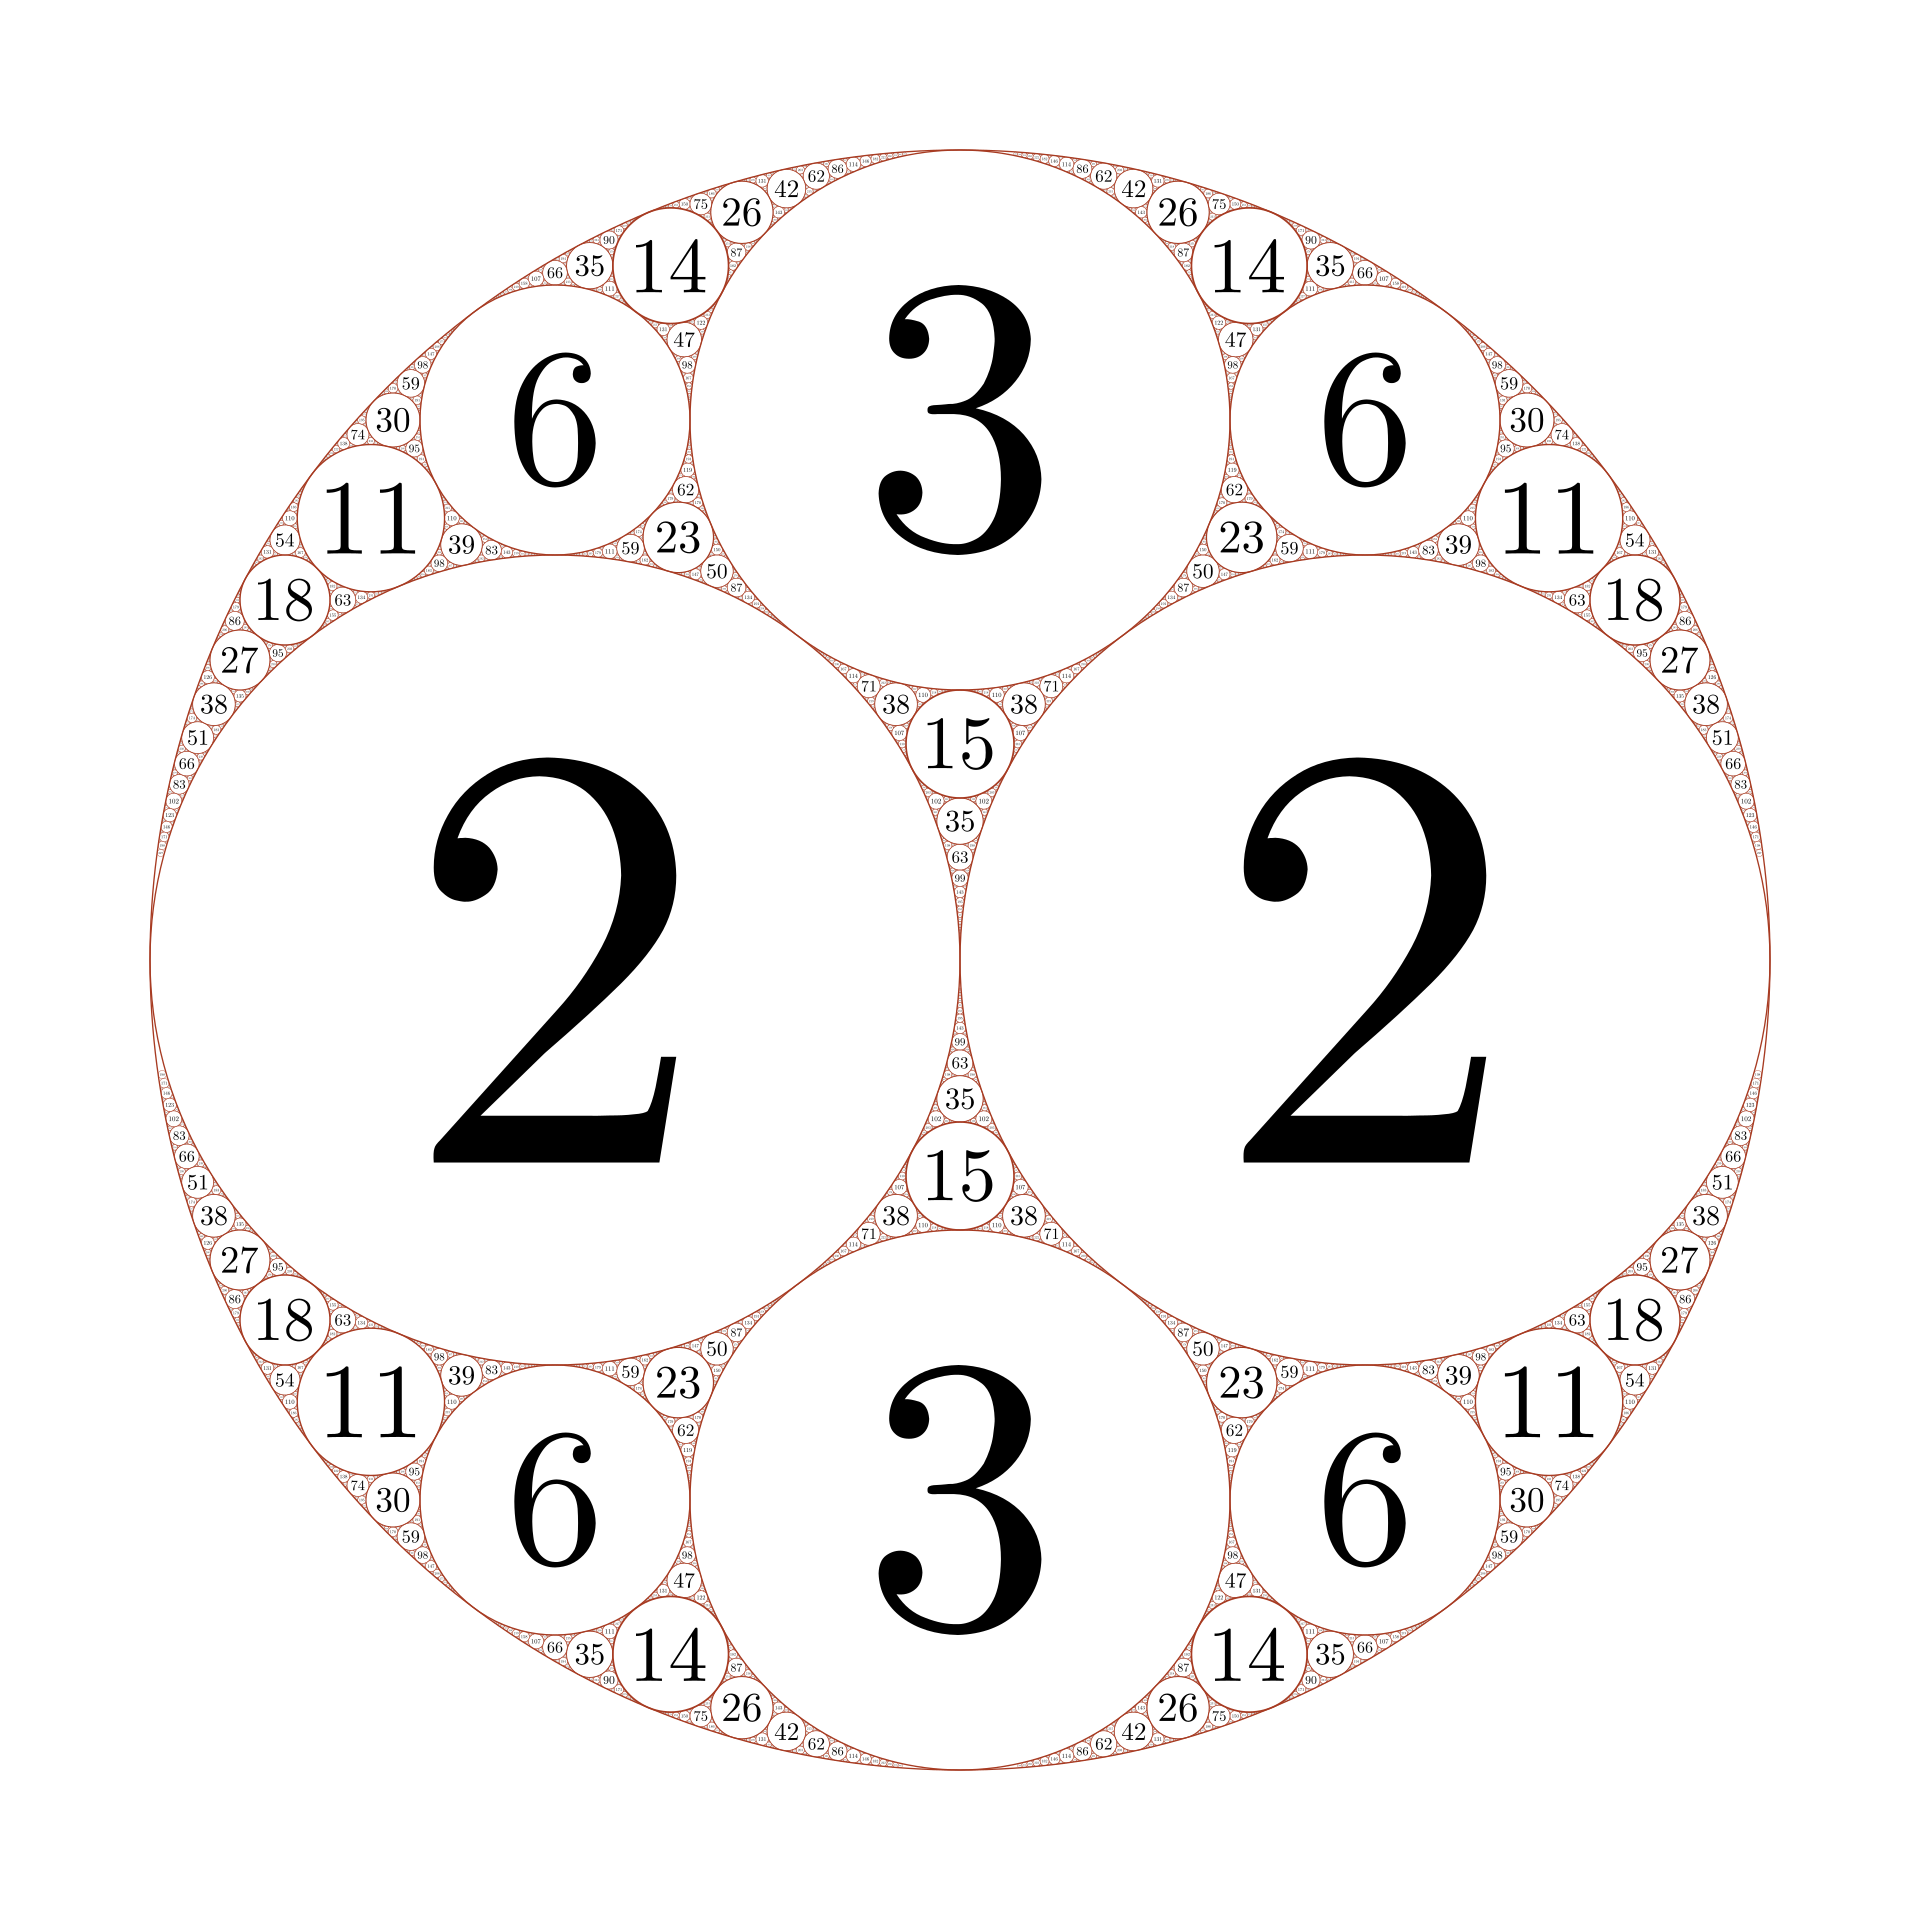
\includegraphics[width=0.3\linewidth]{dikaer.png}
\end{document}
